\documentclass{article}

\usepackage{fullpage}
\usepackage{textcomp}
\usepackage{graphicx}
\usepackage{amsmath}
\usepackage{color}

\renewcommand{\labelenumi}{\arabic{enumi}.}
\renewcommand{\labelenumii}{(\alph{enumii})}

\begin{document}

\begin{center}{\Large\textbf{CSCC01 Team Information}}\end{center}
\begin{center}{\large{\textbf{Group: UofToilets}}}\end{center}

\section{Group Member - Kieran Hansen}
\subsection{Relevant Information}
    Student Number: 1007062474 \newline
    UTORID: hansen20 \newline
    Email: kieran.hansen@mail.utoronto.ca
\subsection{About Me}
\begin{figure}[h]
    \centering
    
\includegraphics[width=0.25\linewidth]{images/KieranPhoto.jpg}
\end{figure}
A dedicated student passionate about learning and technology, I'm always looking for opportunities to better myself and further my understanding of different technologies. I excel in environments where I feel challenged to learn new things and adapt to change. These proficiencies have helped me in the past to assist companies I've worked for with various tasks I may not have initially considered my forte. \newline\par
I look forward to working on this project with the team, and learning more about modern tech stacks and development life cycles in the process! I'm sure my creative vision and organizational skills will contribute to the successful ideation and realization of the app we've been asked to work on!

\noindent\makebox[\linewidth]{\rule{\paperwidth}{0.4pt}}

\section{Group Member - Isaiah Velasquez}
\subsection{Relevant Information}
    Student Number:   \newline
    UTORID:  \newline
    Email: 
\subsection{About Me}

\noindent\makebox[\linewidth]{\rule{\paperwidth}{0.4pt}}

\section{Group Member - Sebastian Jingoi}
\subsection{Relevant Information}
    Student Number: 1009330733 \newline
    UTORID: jingoise \newline
    Email: s.jingoi@mail.utoronto.ca
\subsection{About Me}
\begin{figure}[h]
    \centering
    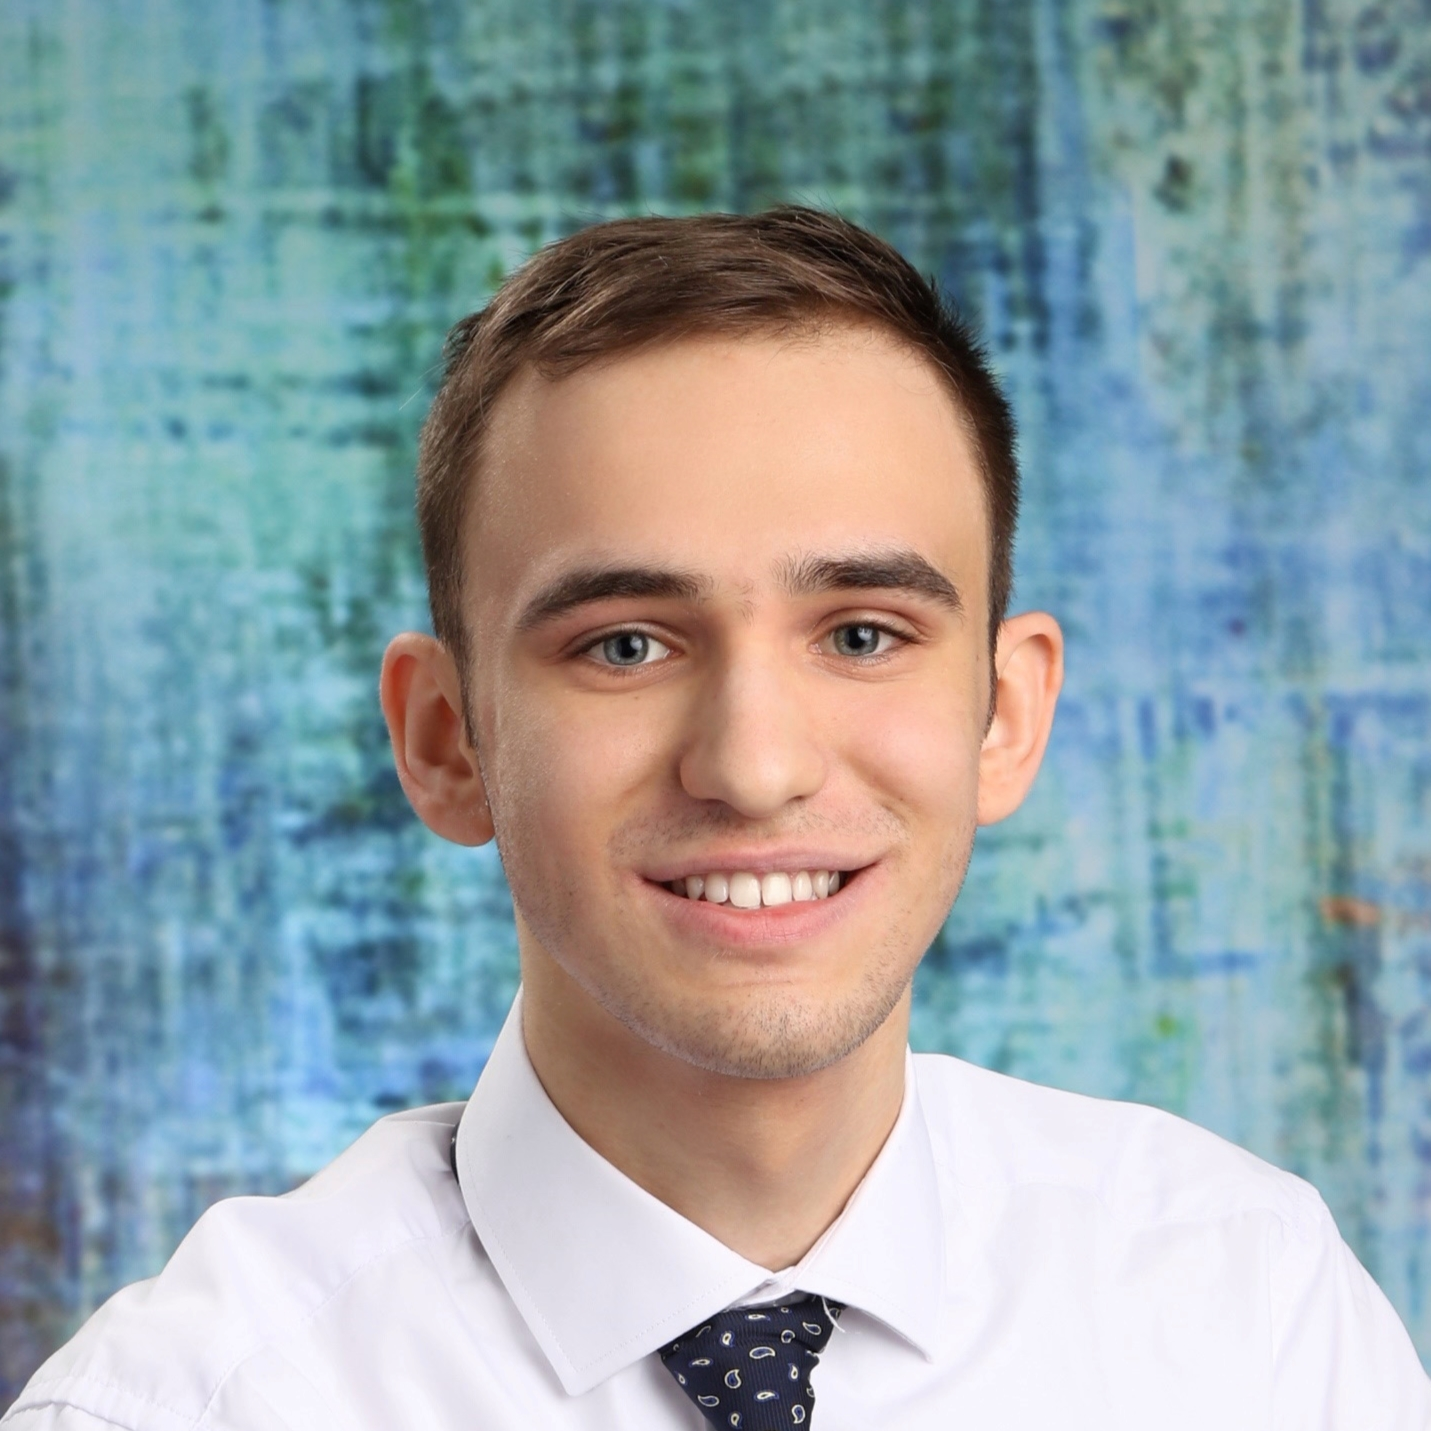
\includegraphics[width=0.25\linewidth]{images/SebPhoto.jpg}
\end{figure}
I am a student who is passionate about the things I create or work on. Whether it be photography, piano, or programming, I make sure to invest my best effort to create the highest quality output. I also ensure that I am always learning something new about technology, and this has been true ever since I was first exposed to computers at a very young age. Projects like these are where I demonstrate the culmination of the knowledge I have gained over time, and I know that this project will continue expanding my understanding.

\noindent\makebox[\linewidth]{\rule{\paperwidth}{0.4pt}}

\section{Group Member - Zain Rizvi}
\subsection{Relevant Information}
    Student Number:  \newline
    UTORID:  \newline
    Email: 
\subsection{About Me}

\noindent\makebox[\linewidth]{\rule{\paperwidth}{0.4pt}}

\section{Group Member - Hriday Algh}
\subsection{Relevant Information}
    Student Number:  \newline
    UTORID:  \newline
    Email: 
\subsection{About Me}

\end{document}
